\chapter{Linearizzazione}
\section{Idea della linearizzazione}
Per capire cosa aspettarci in un intorno di un punto fisso $x_0$ proviamo a linearizzare:
\[\dot x=F(x)=\under{=0}{F(x_0)}+\Dc F(x_0)(x-x_0)+o(\norm{x-x_0}).\]
Se $\norm{x-x_0}$ \`e abbastanza piccolo speriamo di trovare informazioni decentemente affidabili su $F(x)$ vicino a $x_0$ studiando $\Dc F(x_0)$.
\begin{example}[Esempio dove linearizzazione fallisce]
Linearizziamo il sistema dato da $F(x,y)=(x^2,x+y^2)$.
\[\Dc F(0,0)=\rbar{\mat{2x & 0\\ 1 &2y}}_{x=y=0}=\mat{0 & 0\\ 1&0},\]
quindi il sistema linearizzato ha equazione $G(x,y)=(0,x)$.
Problema: il sistema orginale si comporta in modo un po' diverso nell'orgine (acquisto una famiglia di punti fissi, orbite si deformano ecc\dots).
\begin{center}
    \begin{figure}[!htb]
        \centering
        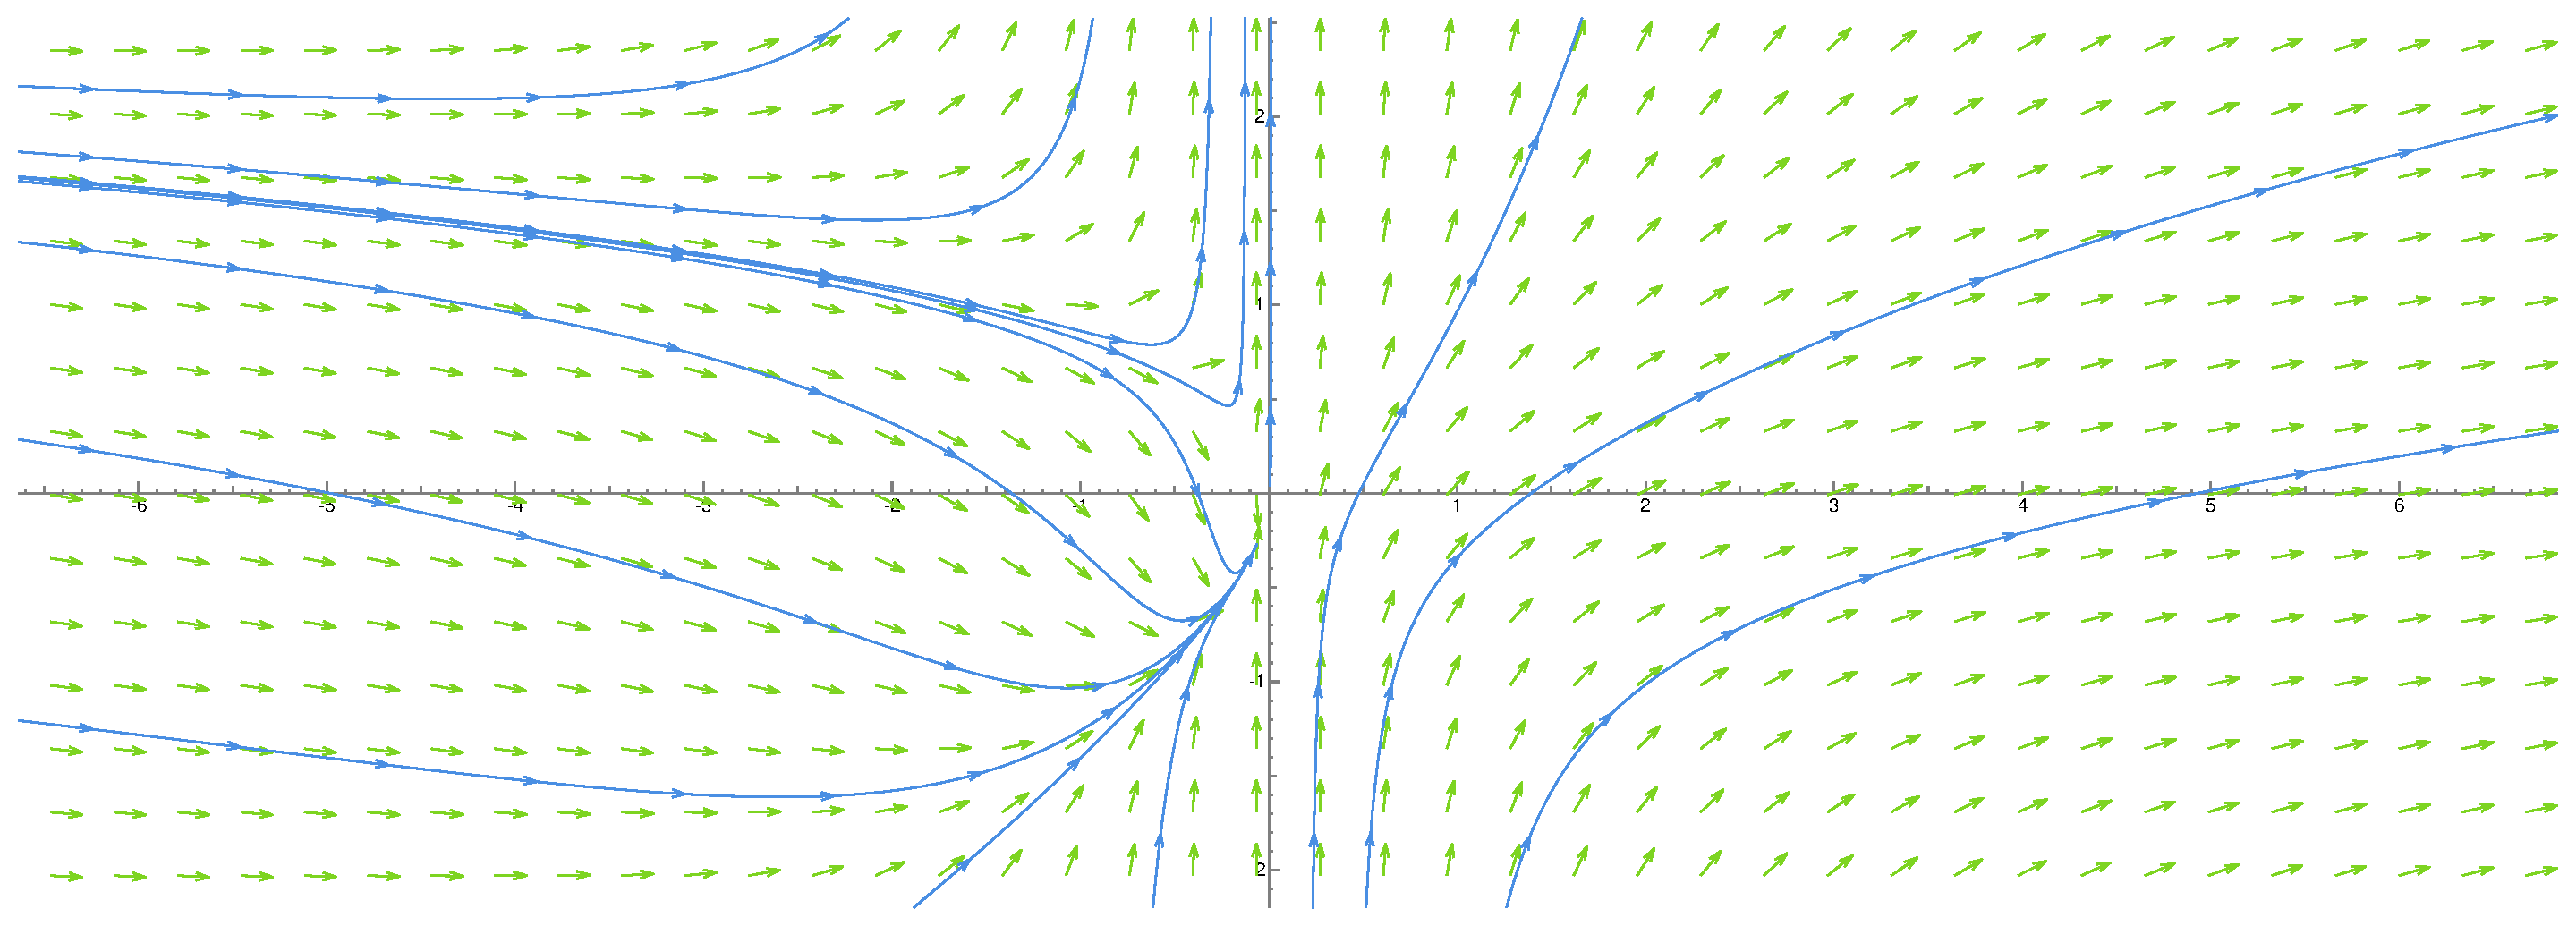
\includegraphics[height=2.8cm]{Immagini/fallita_linearizzazione.pdf}
    \end{figure}
    $\downarrow$
    \begin{figure}[!htb]
        \centering
        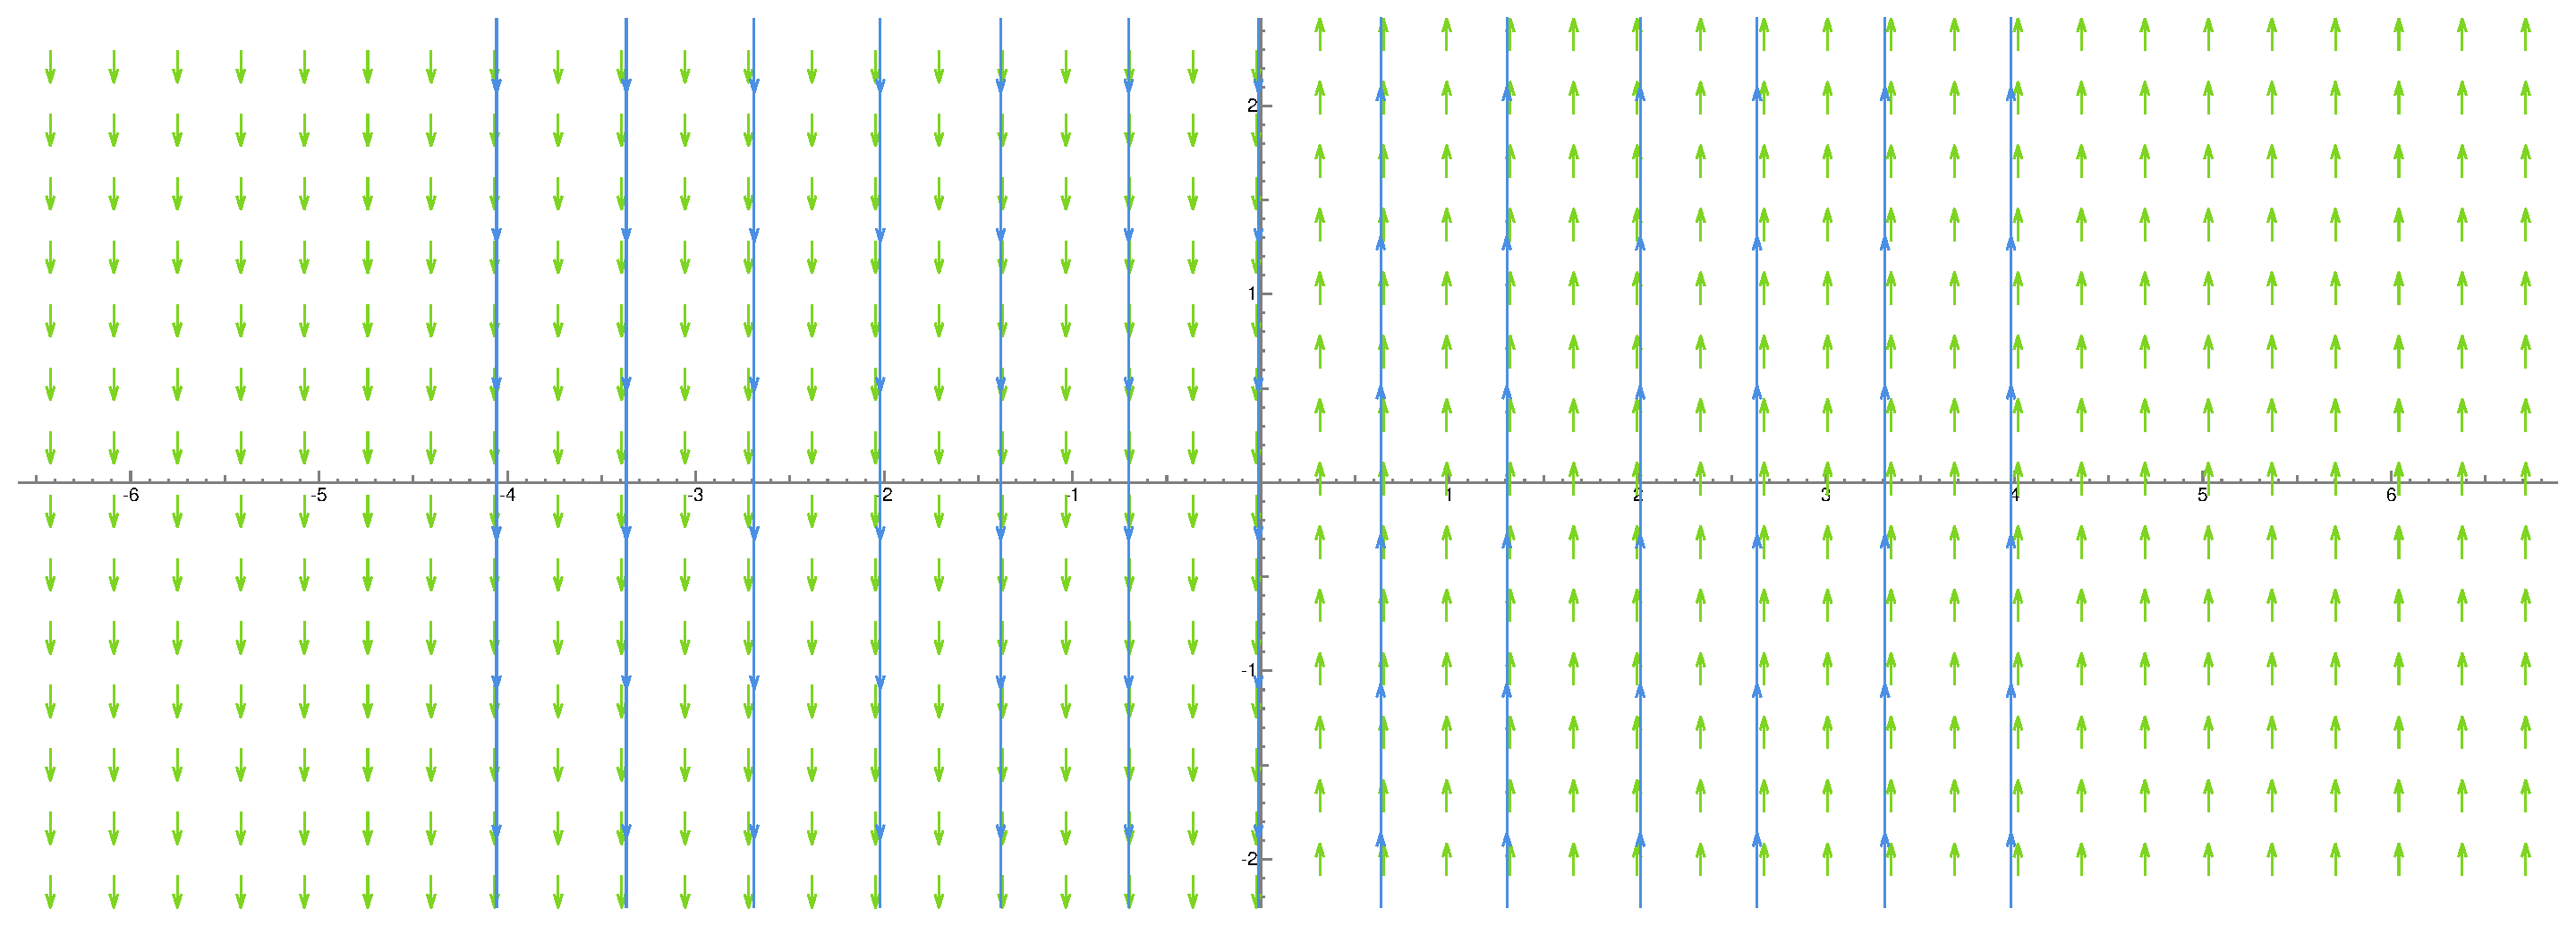
\includegraphics[height=2.8cm]{Immagini/fallita_linearizzazione_linearizzato.pdf}
    \end{figure}
\end{center}



\end{example}

\noindent Possiamo caratterizzare i punti stabili ``adatti allo studio tramite linearizzazione" dando la seguente definizione

\begin{definition}[Punti fissi iperbolici]
Un punto fisso $x_0\in\R^d$ per $F\in C^1$ si dice \textbf{iperbolico} se $\Dc F(x_0)$ non ha autovalori con parte reale nulla.
\end{definition}

\noindent Questi sono i punti ``buoni" perch\'e vale il seguente teorema.

\begin{theorem}[Hartman-Grobman]\label{TeoremaHartmanGrobman}
Sia $x_0\in\R^d$ un punto fisso iperbolico per $\dot x=F(x),\ F\in C^1$ e sia $\phi_t$ il flusso di questo sistema.\\
Consideriamo ora il \textbf{sistema linearizzato in $x_0$}, ovvero il sistema dato da
\[\dot y=\Dc F(x_0) y,\ y\in\R^d\]
e sia $\psi_t$ il flusso di questo sistema.\\
Esistono allora $U$ intorno di $x_0$, $V$ intorno di $0$ e un omeomorfismo $h:U\to V$ tale che per ogni $x\in U$ si ha che per ogni $t$ tale che $\phi_t(x)\in U$
\[h(\phi_t(x))=\psi_t(h(x)).\]
\end{theorem}
\begin{proof}
NON DATA DURANTE IL CORSO.
\end{proof}

\begin{remark}
La condizione $\Real(\la)=0$ \`e equivalente a $\abs{e^\la}=1$, cio\`e $e^\la=e^{i\theta}$. Intuitivamente questo ci dice che l'autospazio generalizzato corrispondente a $\la$ e $\ol\la$ non \`e attratto verso il punto fisso ma non vi \`e neanche respinto nel caso lineare, dunque nel sistema originale la sorte dei punti \`e determinata da espressioni non lineari.
\end{remark}

\begin{remark}
Anche se $F$ ha maggiore regolarit\`a, in generale $h$ non acquista regolarit\`a.
\end{remark}

\noindent
Ricordiamo il seguente
\begin{theorem}[Decomposizione in forma di Jordan reale]\label{JordanReale}
Sia $A\in\Mc(d,\R)$, allora esiste $P\in Mc(d,\R)$ tale che $\det P\neq 0$ e $\Lambda=P\ii AP$ \`e diagonale a blocchi.
\end{theorem}
\noindent
Supponiamo che gli autovalori di $A$ siano in una delle seguenti forme
\begin{itemize}
\item $\{\la_j\}_{j\in\{1,\cdots, k\}}$ con $\la_j\in\R$ e $m_{alg}(\la_j)\leq 3$
\item $\cpa{a_j+ib_j}_{j\in\{1,\cdots, \ell\}}$ con $a_j,b_j\in\R$, $b_j\neq 0$ e $m_{alg}(a_j+ib_j)=1$.
\end{itemize}
Allora $\Lambda=diag(\Lambda_1,\cdots,\Lambda_k,B_1,\cdots,B_\ell)$ con
\begin{align*}
\Lambda_j\in&\cpa{\mat{\la_j & 1 & 0\\ 0&\la_j &1\\ 0&0&\la_j},\ \mat{\la_j & 1 & 0\\ 0&\la_j &0\\ 0&0&\la_j},\ \mat{\la_j & 0 & 0\\ 0&\la_j &0\\ 0&0&\la_j}}\cup\\
&\cup\cpa{\mat{\la_j & 1\\0&\la_j},\ \mat{\la_j&0\\0&\la_j},\mat{\la_j}}
\end{align*}
\[B_j=\mat{a_j & -b_j\\ b_j & a_j}.\]
Osserviamo che se $\dot y=\Dc F(x_0)y$ ed esiste $P$ invertibile tale che $P\ii \Dc F(x_0)P=\Lambda$ con $\Lambda$ in forma di Jordan reale allora, ponendo $z=P\ii y$ troviamo un omeomorfismo tale che
\[\dot z=P\ii \dot y=P\ii \Dc F(x_0)y=(P\ii\Dc F(x_0)P)z=\Lambda z.\]
\begin{notation}
Sia $V_{\la_j}$ l'autospazio generalizzato di $\la_j$, similmente per $a_j+ib_j$.
\end{notation}

\begin{proposition}[Gli autospazi generalizzati sono invarianti]\label{AutospaziGeneralizzatiSonoInvarianti}
Per $\dot y=Ay$, $A\in\Mc(d,\R)$ si ha che $V_{\la_j}$ e $V_{a_j+ib_j}$ sono insiemi invarianti.
\end{proposition}
\begin{proof}
Senza perdita di generalit\`a supponiamo che $A=\Lambda$ sia in forma di Jordan reale e a meno di permutare le coordinare mostriamo la tesi solo per $V_{\la_1}$\footnote{dove $\la_1$ in questo caso si riferisce ad autovalori potenzialmente complessi.}. Osserviamo che un generico vettore di $V_{\la_1}$ \`e della forma $y_0=((y_0)_1,\cdots, (y_0)_s, 0,\cdots, 0)$, dove $s=m_{alg}(\la_1)$ (dove poniamo $s=2$ nel caso di autovalore complesso). La tesi segue calcolando: 
\[\phi_t(y_0)=e^{t\Lambda}y_0=diag(e^{\Lambda_1 t},\cdots e^{\Lambda_s t})y_0=\mat{e^{\Lambda_1 t}\mat{(y_0)_1\\\vdots\\(y_0)_s}\\0\\\vdots\\0}\in V_{\la_1}.\]
\end{proof}

\begin{definition}[Sottospazi stabili]
Il \textbf{sottospazio stabile} di $0$ per il sistema $\dot y=Ay$ \`e l'insieme
\[E^s(0)=\Span(v\in V_{\la_i}\mid \Real(\la_i)<0).\]
Il \textbf{sottospazio instabile} ($E^u(0)$) e il \textbf{sottospazio centrale} ($E^c(0)$) sono definiti in modo analogo considerando $\Real(\la_i)>0$ e $\Real(\la_i)=0$ rispettivamente.
\end{definition}

\begin{theorem}[Invarianza e caratterizzazione dei sottospazi stabili]
Dato il sistema $\dot y=Ay$ si ha che:
\begin{enumerate}
\item $\dim E^u(0)+\dim E^s(0)+\dim E^c(0)=d$
\item $E^{s,c,u}(0)$ \`e invariante per $\phi_t$
\item $E^s(0)=\cpa{y_0\in\R^d\mid \displaystyle\lim_{t\to+\infty}\phi_t(y)=0}$
\item $E^u(0)=\cpa{y_0\in\R^d\mid \displaystyle\lim_{t\to-\infty}\phi_t(y)=0}$.
\end{enumerate}
\end{theorem}
\begin{proof}[Dimostrazione. (NON DATA DURANTE IL CORSO)]
Il primo punto segue da noti risultati sugli autospazi generalizzati.\\
Il secondo punto \`e una conseguenza dell'invarianza degli autospazi (\ref{AutospaziGeneralizzatiSonoInvarianti}).\\
Gli ultimi due punti seguono da come funzionano i $e^{\Real(\la)t}$ (questi fattori appaiono dopo essersi portati in forma di Jordan).
\end{proof}

\newpage
\section{Pozzi e Sorgenti}

\begin{definition}[Pozzi e sorgenti]
    Sia $x_0$ un punto fisso. Esso si dice
    \setlength{\leftmargini}{0.5cm}
    \begin{itemize}
        \item \textbf{pozzo} se ogni autovalore di $\Dc F(x_0)$ ha parte reale negativa,
        \item \textbf{sorgente} se ogni autovalore di $\Dc F(x_0)$ ha parte reale positiva.
    \end{itemize}
\end{definition}
    
\begin{remark}
    Si pu\`o pensare a sorgenti come pozzi per tempi negativi.
\end{remark}
    
\begin{proposition}[Stabilit\`a dei pozzi]\label{StabilitaPozzi}
    I pozzi sono asintoticamente stabili
\end{proposition}
\begin{proof}
    A meno di traslare il sistema supponiamo $x_0=0\in\R^d$.\\
    Poich\'e cambi di base lineari non cambiano la stabilit\`a dell'origine supponiamo che $\Dc F(0)$ sia in forma di Jordan reale. Trattiamo prima i casi dove $\Dc F(0)$ consiste di un solo blocco di Jordan e poi uniamo i risultati.
    \setlength{\leftmargini}{0cm}
    \begin{itemize}
        \item[$\boxed{\la\in\R}$] 
        Supponiamo che
        \[\Dc F(0)=\mat{
        \la & 1    &      &\\
            &\ddots&\ddots&\\
            &       &\la & 1\\
            &       &    &\la 
        }\implies \dot x=F(x)=\under{=0}{F(0)}+\Dc F(0)x+O(\norm x^2).\]
        Dato $\e>0$ consideriamo il cambio di base
        \[y=(y_1,\cdots, y_d),\quad y_i=\e^{-i+1}x_{i},\]
        da cui
        \[\dot y=A y+\wt G(y),\quad A=\mat{
        \la & \e    &      &\\
            &\ddots&\ddots&\\
            &       &\la & \e\\
            &       &    &\la 
        },\ {\wt G(y)}=O(\norm y^2).\]
        Affermiamo che la funzione
        \[V(y)=\frac12 \norm y^2\]
        \`e di Lyapunov stretta in un intorno di $0$. La prima condizione \`e evidentemente verificata, quindi dobbiamo solo trovare un intorno dove $\dot V(y)<0$ per $y\neq 0$.
        \begin{align*}
            \dot V(y)=&\sum_{i=1}^{d-1}y_i\under{\dot y_i}{(\la y_i+\e y_{i+1}+\wt G_i(y))}+y_d\under{\dot y_d}{(\la y_d+\wt G_d(y))}=\\
            =&\la\norm y+\e \sum_{i=1}^{d-1}y_iy_{i+1}+{y\cdot \wt G(y)}\leq\\
            \leq& \la\norm y+\frac\e2 \pa{\sum_{i=1}^{d-1}y_i^2 +\sum_{i=2}^{d}y_i^2}+O(\norm y^3)=\\
            =&\pa{\la+\frac\e2}(y_1^2+y_d^2)+(\la+\e)\sum_{i=2}^{d-1}y_i^2+O(\norm y^3)\leq\\
            \leq& (\la+\e)\norm y^2+O(\norm y^3).
        \end{align*}
        Cerchiamo dunque condizioni valide per $\e$ e $\norm y$:\\
        Poich\'e $\la<0$ \`e lecito fissare $\e\in(0,\abs\la)$. Per le propriet\`a degli $O$ grandi esistono $r,C>0$ tali che
        \[\norm y<r\implies \dot V(y)\leq((\la+\e)+C\norm y)\norm y^2.\]
        Ponendo ora $\la+\e+C\norm y<0$ si ha che se 
        \[r'<\min\cpa{r,\frac{\abs{\la+\e}}{C}}\]
        allora per $y\in B_{r'}(0)\bs\cpa0$ vale
        \[\dot V(y)\leq ((\la+\e)+C\norm y)\norm y^2<0,\]
        cio\`e $V$ \`e una funzione di Lyapunov stretta per $x_0$ in un opportuno cambio di base, dunque $x_0$ \`e asintoticamente stabile per il secondo teorema di Lyapunov (\ref{TeoremaLyapunov2AsintoticaStabilita}).
        \item[$\boxed{\la\in\C\bs \R}$] Supponiamo che
        \[\Dc F(0)=\mat{
        \emat{a&b\\-b&a} & \emat{1&0\\0&1}     &      \\
            &\ddots &\ddots&\\
            &       &\ddots
        }\]
        A meno di un coniugio troviamo
        \[\dot y=Ay+\wt G(y),\quad A=\mat{
        \emat{a&b\\-b&a} & \emat{\e&0\\0&\e}     &      \\
            &\ddots &\ddots&\\
            &       &\ddots
        }\]
        e concludiamo in modo simile al caso precedente.
        \item[$\boxed{\text{generale}}$] Segue dai due casi precedenti dando un ulteriore limitazione con gli $O$ grandi sui termini non lineari.
    \end{itemize}
    \setlength{\leftmargini}{0.5cm}
\end{proof}

\section{Classificazione dei punti stabili lineari sul piano}
Consideriamo i sistemi lineari di questa forma
\[\dot x=Ax,\quad A\in\Mc(2,\R),\ x=\mat{u\\ v}\in\R^2.\]
Sappiamo che
\[\phi_t(x_0)=e^{At}x_0,\]
in particoalre $x_0=0$ \`e un punto fisso.
\[A=\mat{a & b\\ c & d}\implies p_A(\la)=\la^2-(a+d)\la+ad-bc=\la^2-(\tr A)\la+\det A.\]
Segue che gli autovalori di $A$ sono
\[\la_{\pm}=\frac{\tr A\pm \sqrt{\Delta}}{2},\ \Delta=(\tr A)^2-4\det A.\]
Consideriamo i possibili casi:
\setlength{\leftmargini}{0cm}
\begin{itemize}
\item[$\boxed{\emat{\det A>0\\ \Delta>0}}$] Gli autovalori $\la_\pm$ sono reali distinti.\\
$\star)$ Se $\tr A>0$ allora $\la_+>\la_->0$, da cui a meno di coniugio
\[A=\mat{\la_+ &0\\0&\la_-}\implies \begin{cases}
\dot u=\la_+ u\\
\dot v=\la_- v
\end{cases},\]
da cui le soluzioni sono
\[(u(t), v(t))=(e^{\la_+t}u_0, e^{\la_-t}v_0).\]
Questa situazione \`e detta \textbf{nodo instabile}.\\ Osserviamo che $E^u(0)=\R^2$ e $E^s(0)=E^c(0)=\cpa0$.\\
$\star)$ Se $\tr A<0$ allora $\la_-<\la_+<0$ e troviamo il \textbf{nodo stabile}.\\ Osserviamo che $E^s(0)=\R^2$ e $E^u(0)=E^c(0)=\cpa0$.
\item[$\boxed{\emat{\det A>0\\ \Delta<0}}$] Gli autovalori $\la_\pm$ sono complessi coniugati. $\la_\pm=\al\pm i\beta$ con $\al,\beta\in\R$. Segue che $\tr A=2\al$. A meno di coniugio
\[A=\mat{\al & -\beta\\ \beta &\al}\implies e^{At}=e^{\al t}\mat{\cos(\beta t) & -\sin(\beta t)\\ \sin(\beta t) & \cos(\beta t)}.\]
$\star)$ Se $\al>0$ troviamo
\[x(t)=e^{\al t} R_{\beta t}(x_0)\]
cio\`e un \textbf{fuoco instabile}. Osserviamo che $E^u(0)=\R^2$ e $E^s(0)=E^c(0)=\cpa0$.\\
$\star)$ Se $\al<0$ troviamo
\[x(t)=e^{\al t} R_{\beta t}(x_0)\]
cio\`e un \textbf{fuoco stabile}. Osserviamo che $E^s(0)=\R^2$ e $E^u(0)=E^c(0)=\cpa0$.\\
$\star)$ Se $\al=0$ troviamo
\[x(t)=R_{\beta t}(x_0)\]
cio\`e un \textbf{centro}. Osserviamo che $E^c(0)=\R^2$ e $E^s(0)=E^u(0)=\cpa0$.
\item[$\boxed{\emat{\det A>0\\ \Delta=0}}$] Gli autovalori coincidono e sono della forma $\la=\tr A/2$. A meno di coniugio abbiamo due possibilit\`a:
\[A=\mat{\la &0\\0&\la}\implies x(t)=e^{\la t}x_0\]
Questa situazione \`e detta \textbf{Stella stabile/instabile} per segno negativo o positivo della traccia rispettivamente.
\[A=\mat{\la & 1\\ 0 &\la}\implies x(t)=e^{\la t}(u_0+t v_0, v_0).\]
Questa situazione \`e detta \textbf{nodo stabile/instabile improprio}.
\item[$\boxed{\emat{\det A<0\\ \Delta>0}}$] Gli autovalori sono reali di segno opposto $\la_-<0<\la_+$. A meno di coniugio
\[A=\mat{\la_+ &0\\ 0&\la_-}\implies x(t)=(u_0e^{\la_+t},v_0e^{\la_-t}).\]
Troviamo un \textbf{punto di sella}. Il segno della traccia specifica solo verso quale asse le iperboli sono schiacciate.\\
Osserviamo che $E^s(0)=\{x=0\},\ E^u(0)=\cpa{y=0},\ E^c(0)=0$, cio\`e lo ``spazio tangente" in $0$ si decompone in una retta stabile e una instabile.
\item[$\boxed{\det A=0}$] Gli autovalori sono $0$ e $\tr A$. In tutti i casi a meno di coniugio una coordinata resta costante, dunque troviamo delle \textbf{rette}.
\end{itemize}

\noindent Riassumiamo i casi nella seguente tabella
\begin{center}
\begin{tabular}{|c|c|c||c|}
\hline
$\sgn\det A$ & $\sgn \Delta$ & $\sgn \tr A$ & Nome\\\hline\hline
+ & + & + & Nodo instabile \\\hline
+ & + & - & Nodo stabile \\\hline
+ & - & + & Fuoco instabile \\\hline
+ & - & - & Fuoco stabile \\\hline
+ & - & 0 & Centro \\\hline
+ & 0 & + & Stella o nodo improprio instabile \\\hline
+ & 0 & - & Stella o nodo improprio stabile \\\hline
- & + & $\bullet$ & Punto di Sella \\\hline
0 & $\bullet$ & $\bullet$ & Rette \\\hline
\end{tabular}
\end{center}

\begin{figure}[!htb]
    \centering
    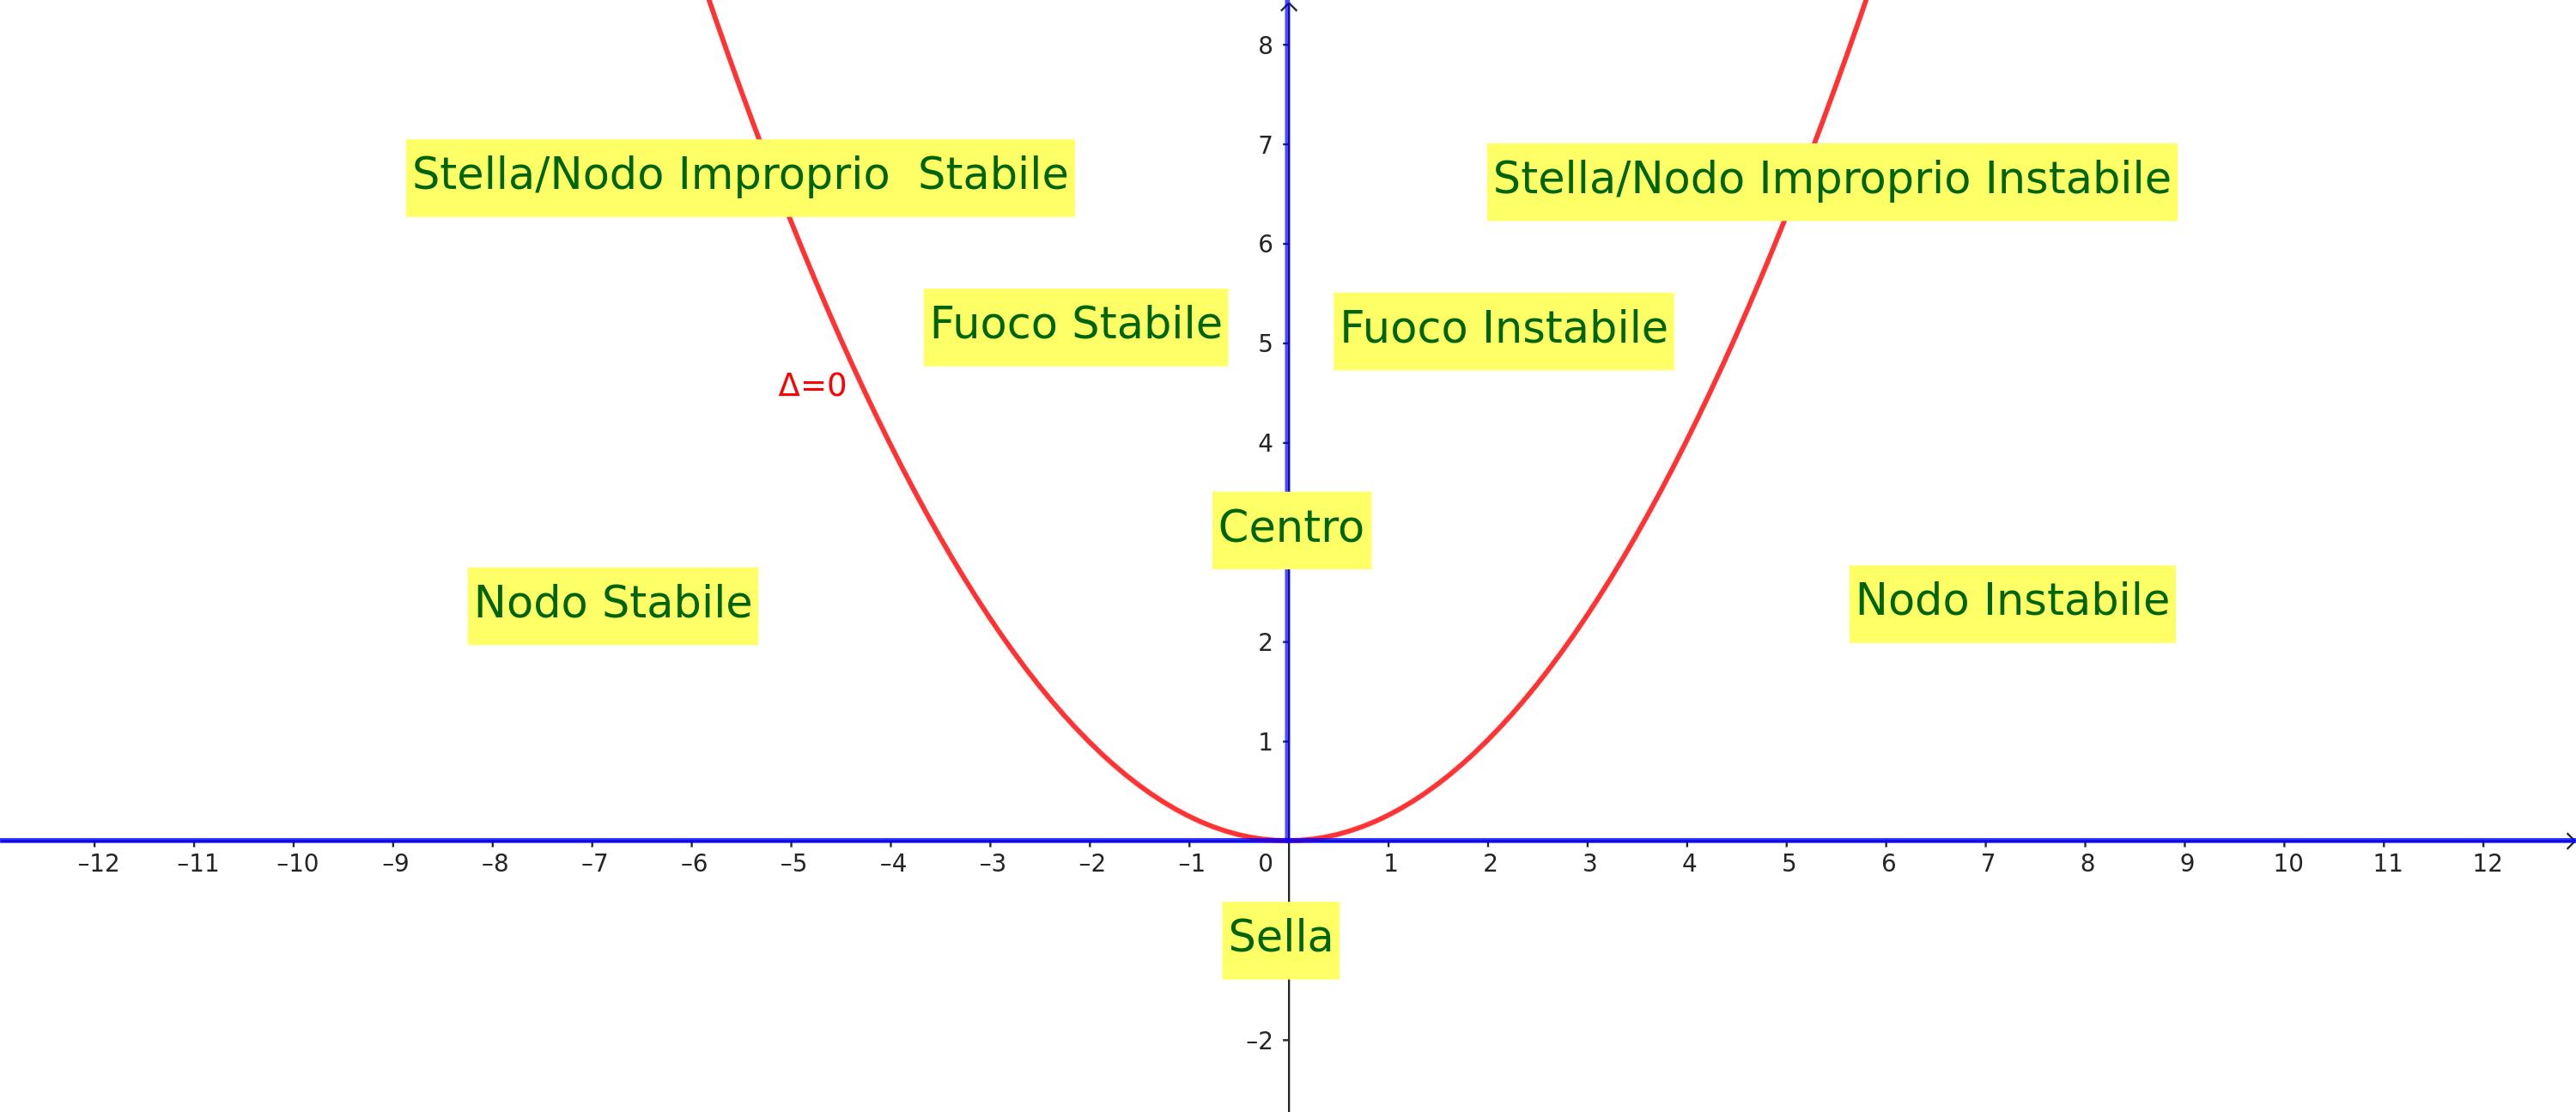
\includegraphics[width=\textwidth]{Immagini/Diagramma_punti_stabili_lineari.png}
    \caption{Utile diagramma che organizza i tipi di punti stabili lineari. L'asse $x$ corrisponde ai possibili valori di $\tr A$ e l'asse $y$ ai possibili valori di $\det A$. La parabola rossa indica il luogo dove $\Delta=0$; nella regione sopra la parabola troviamo $\Delta<0$ e sotto $\Delta>0$. In blu sono indicati i valori di $\tr A$ e $\det A$ per cui il punto stabile in considerazione NON \`e iperbolico.}
\end{figure}

\noindent Riportiamo dei diagrammi di fase per evidenziale la forma delle orbite.

\begin{figure}[!htb]
    \centering
    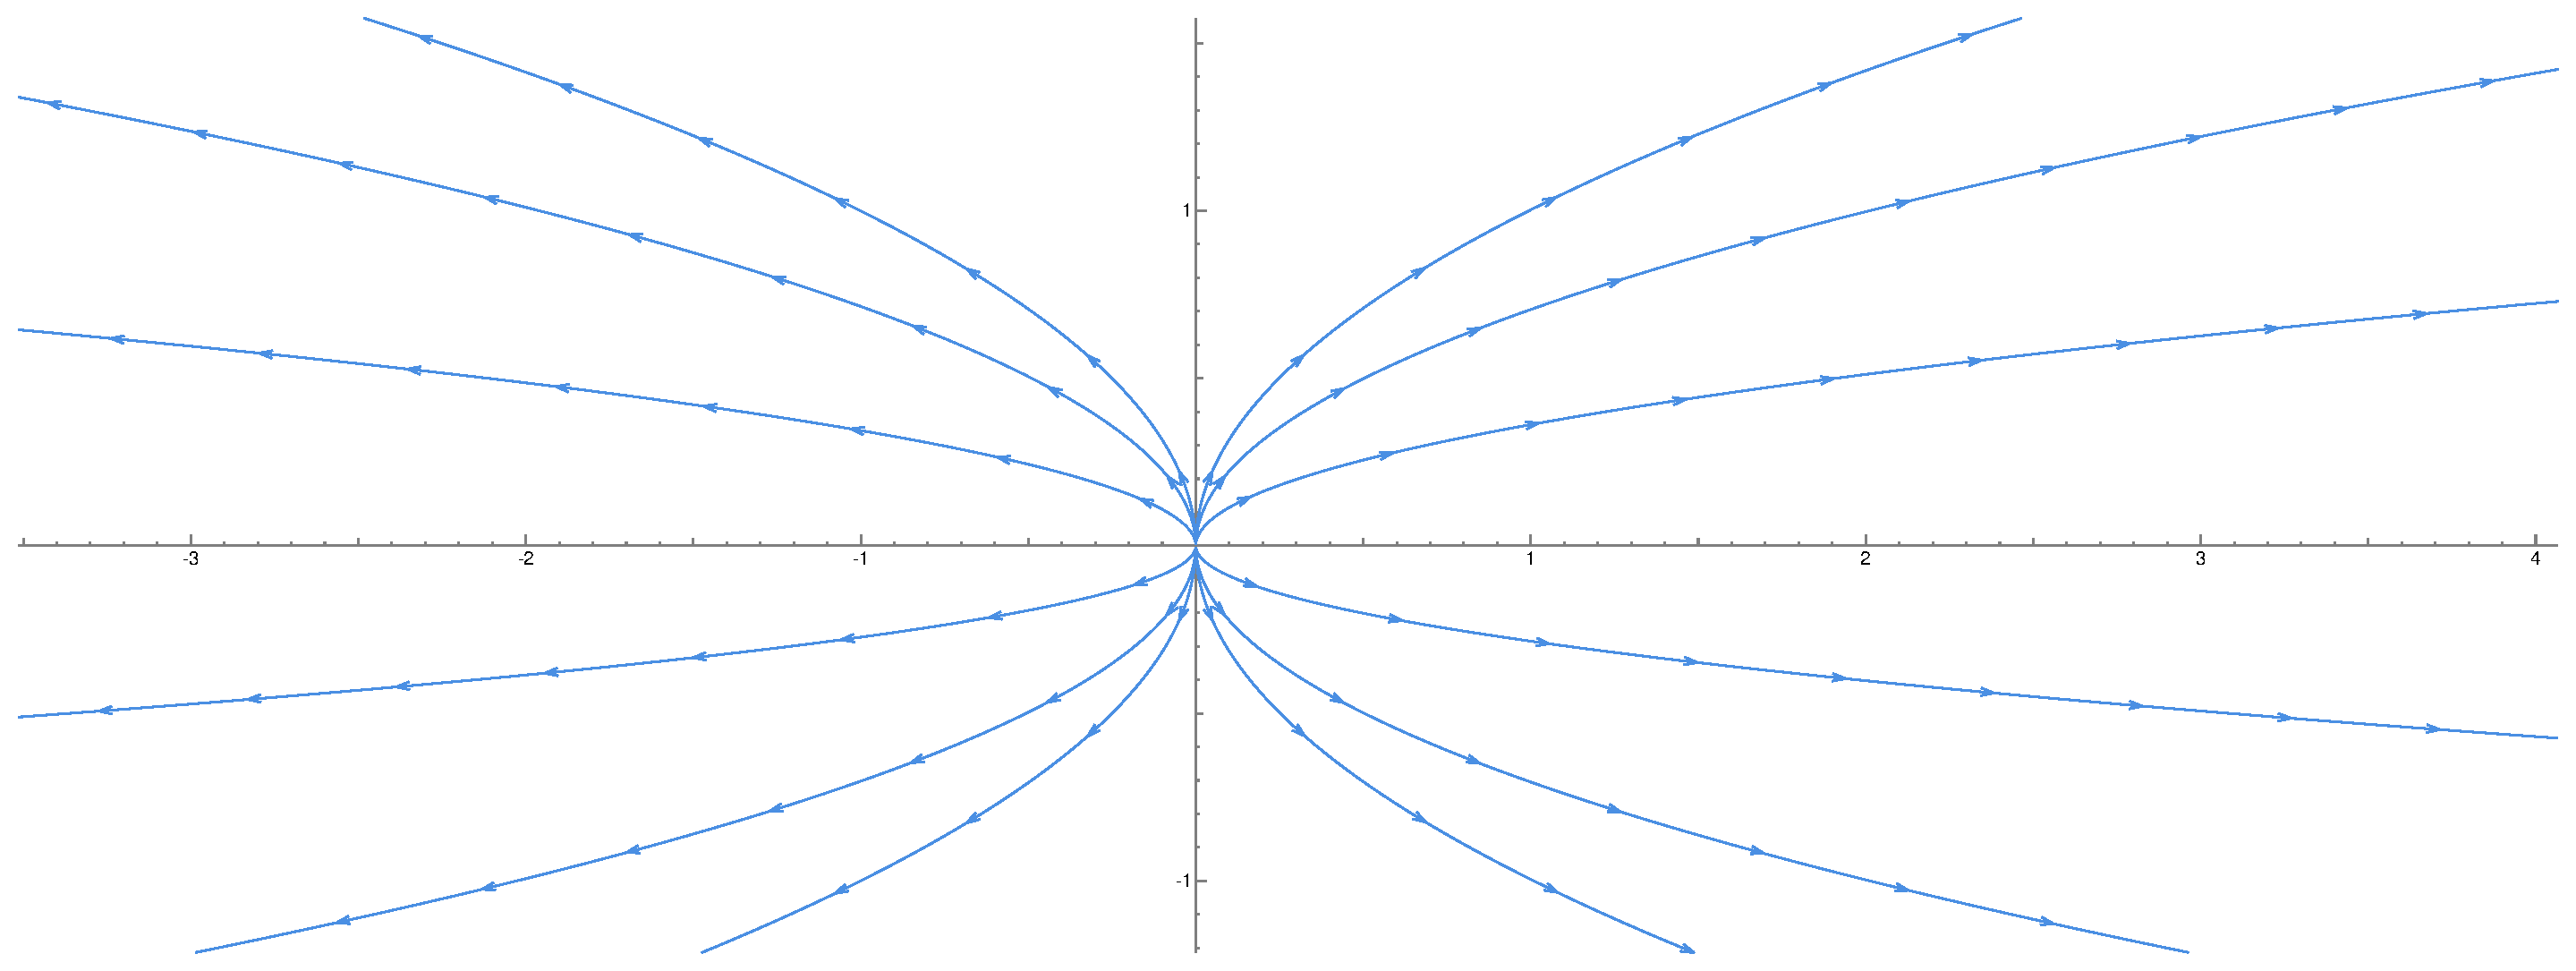
\includegraphics[width=11cm]{Immagini/nodo_instabile.pdf}
    \caption{Nodo instabile}
\end{figure}


\begin{figure}[!htb]
    \centering
    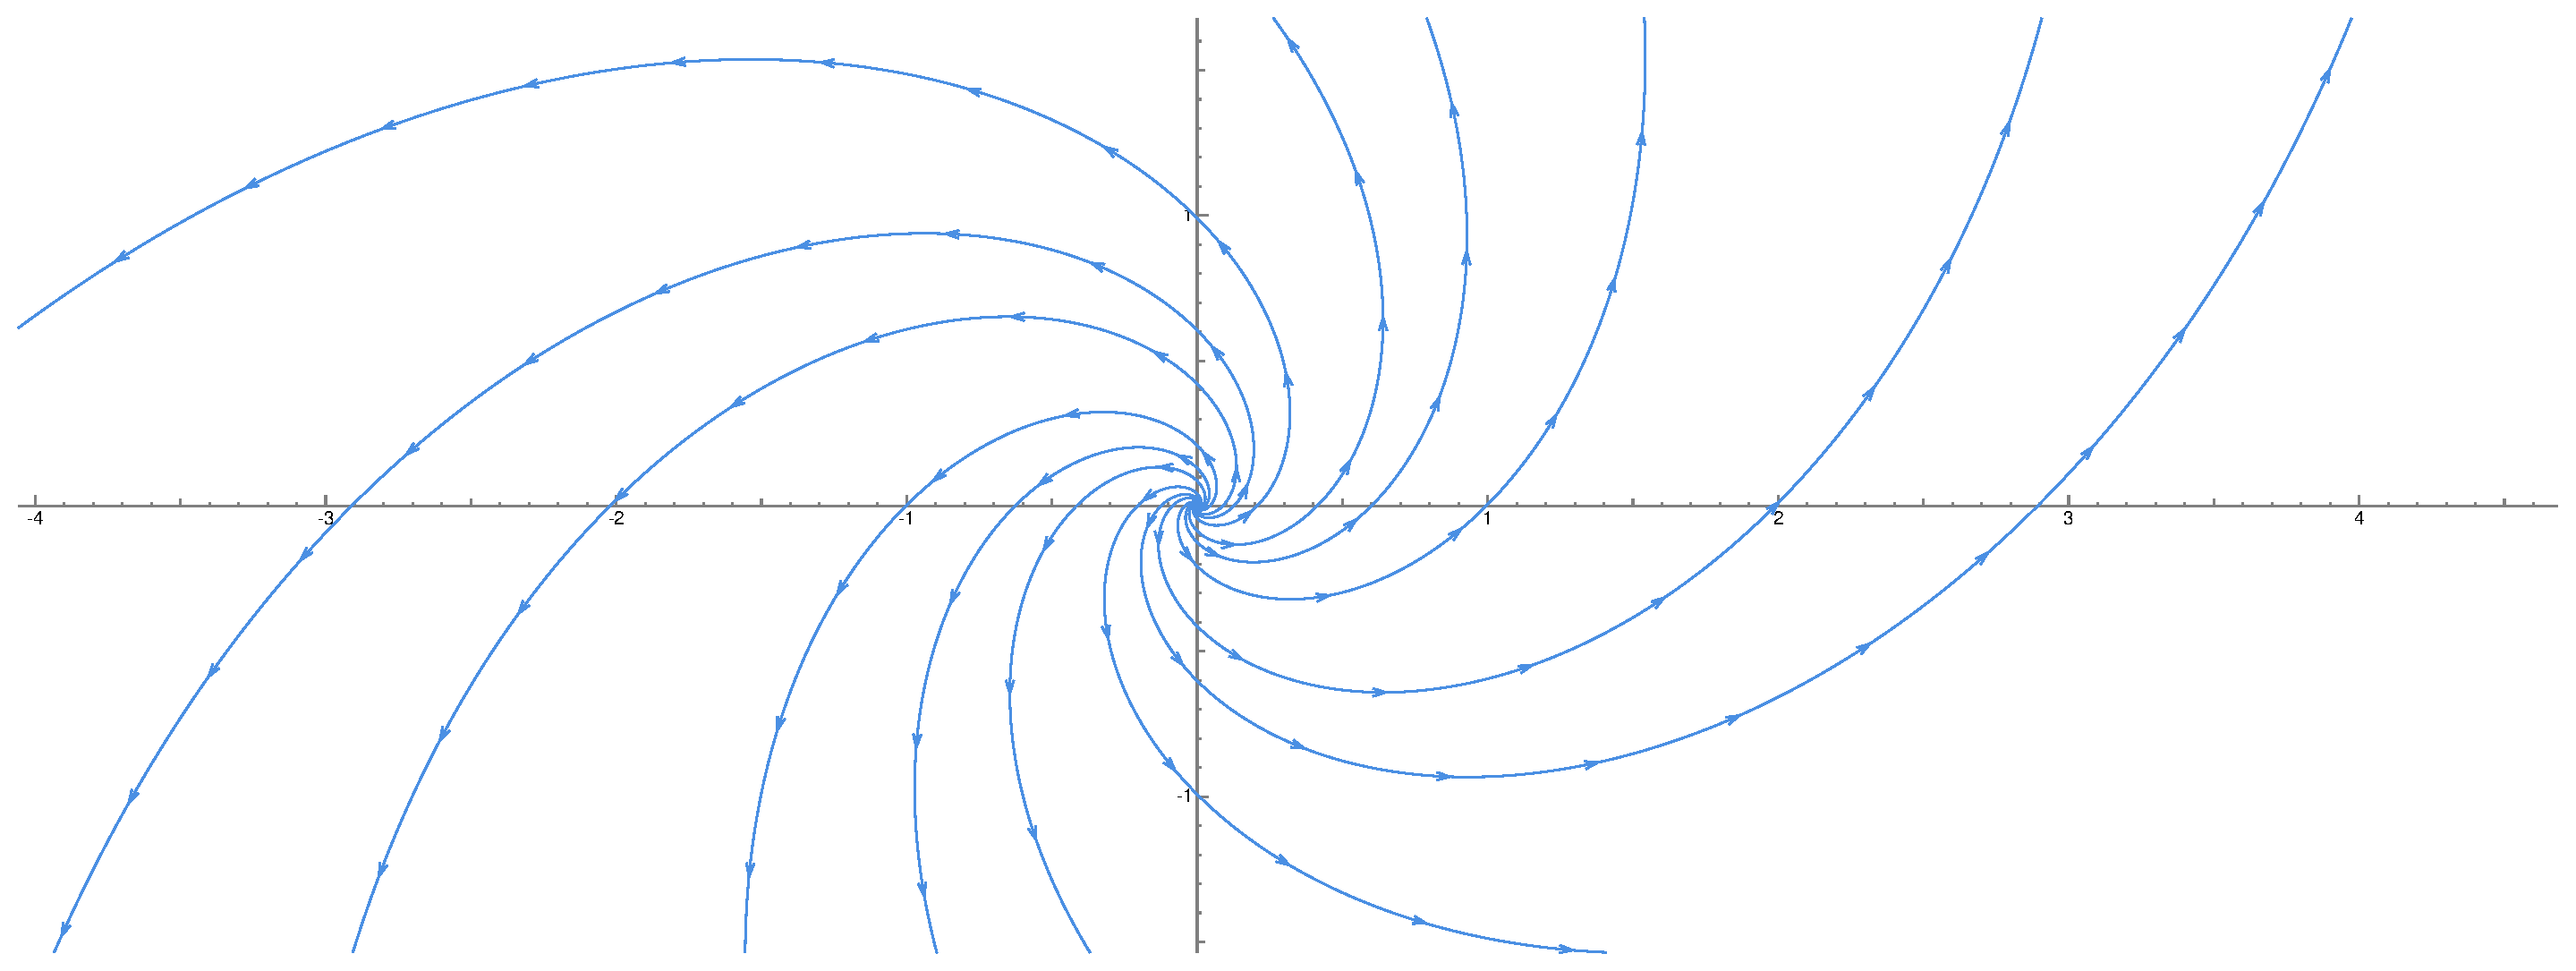
\includegraphics[width=11cm]{Immagini/fuoco_instabile.pdf}
    \caption{Fuoco instabile}
\end{figure}


\begin{figure}[!htb]
    \centering
    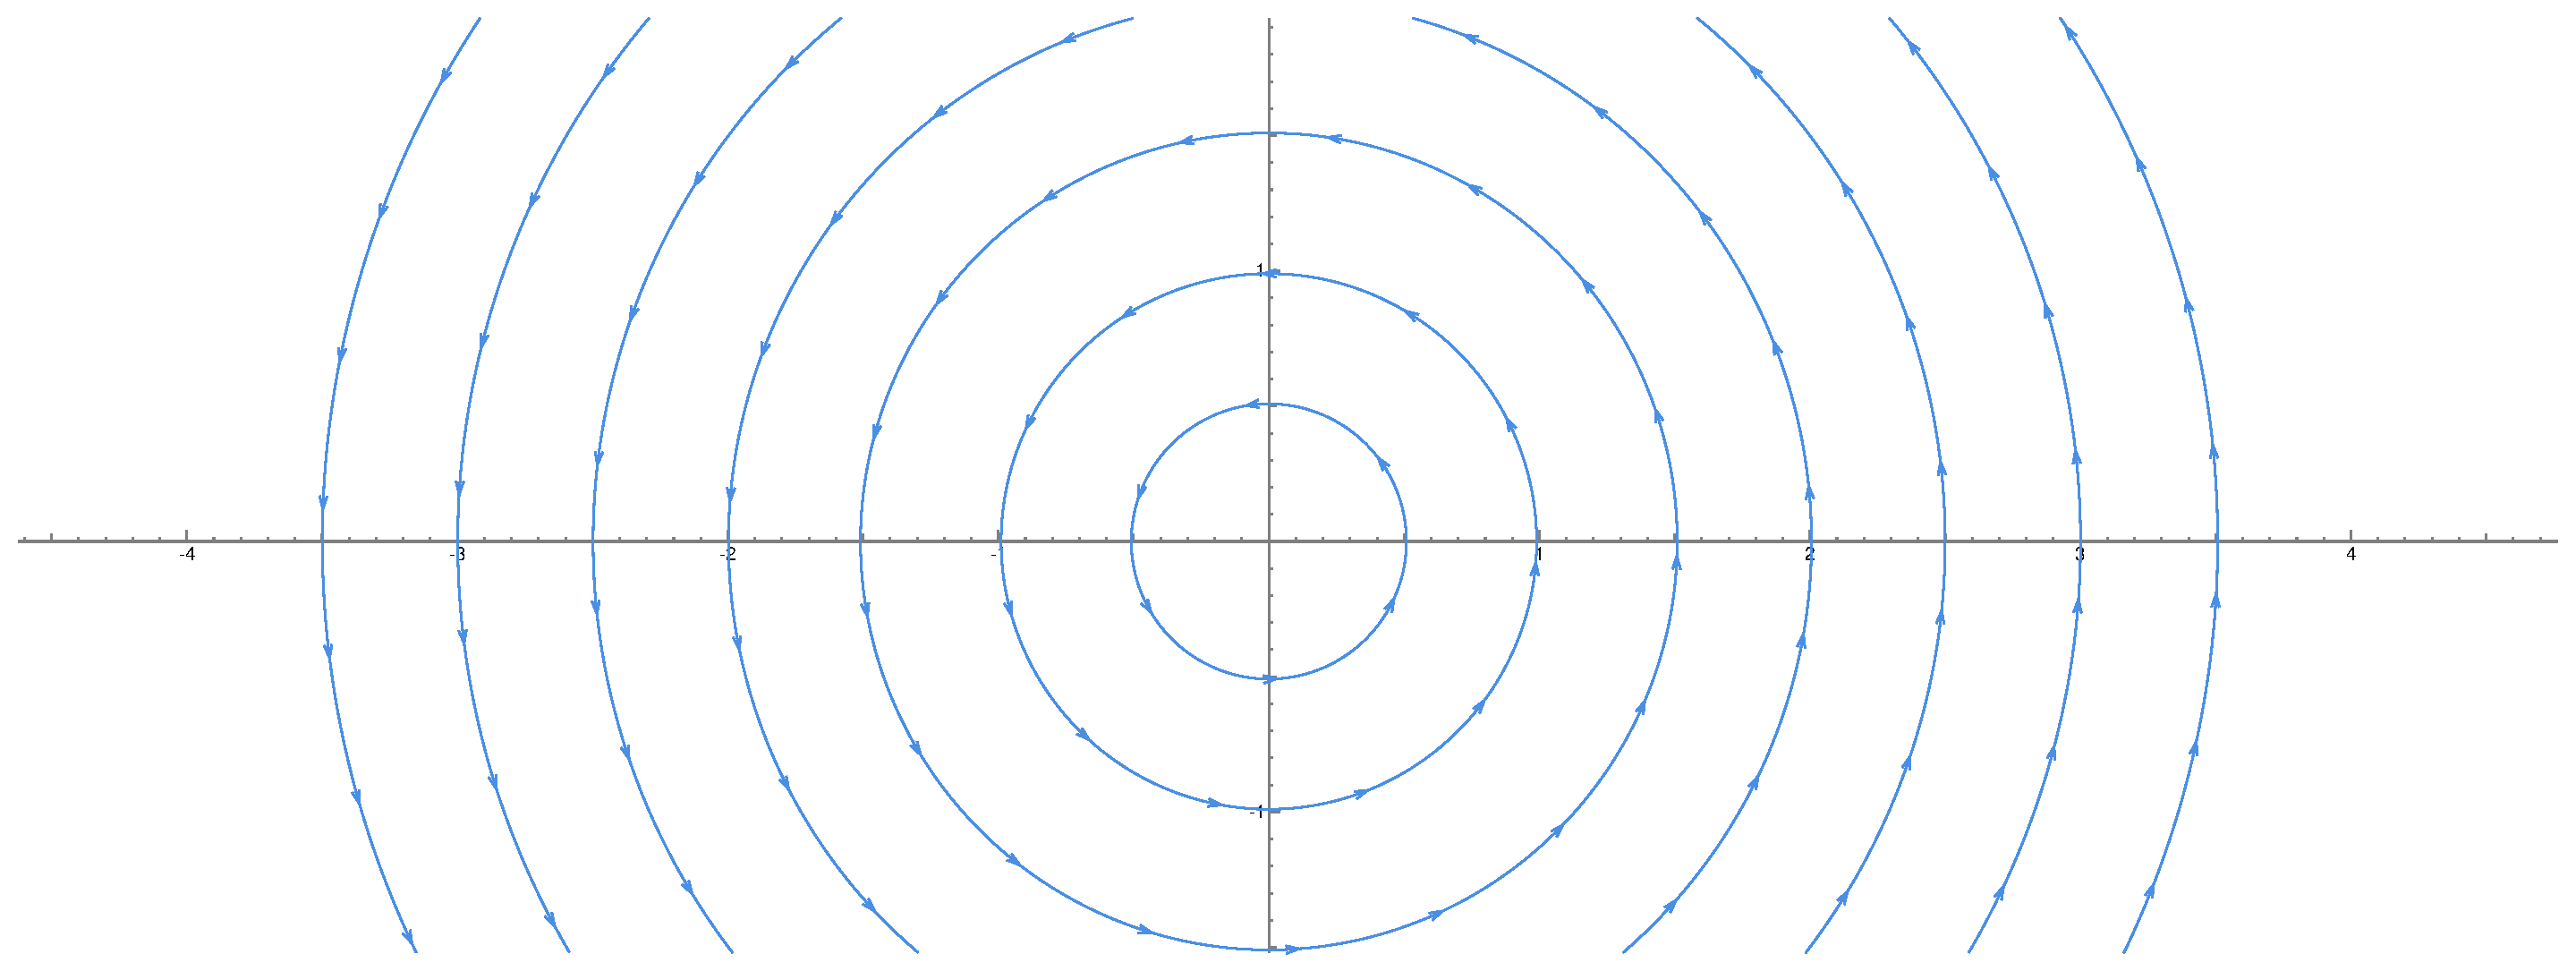
\includegraphics[width=11cm]{Immagini/centro.pdf}
    \caption{Centro}
\end{figure}


\begin{figure}[!htb]
    \centering
    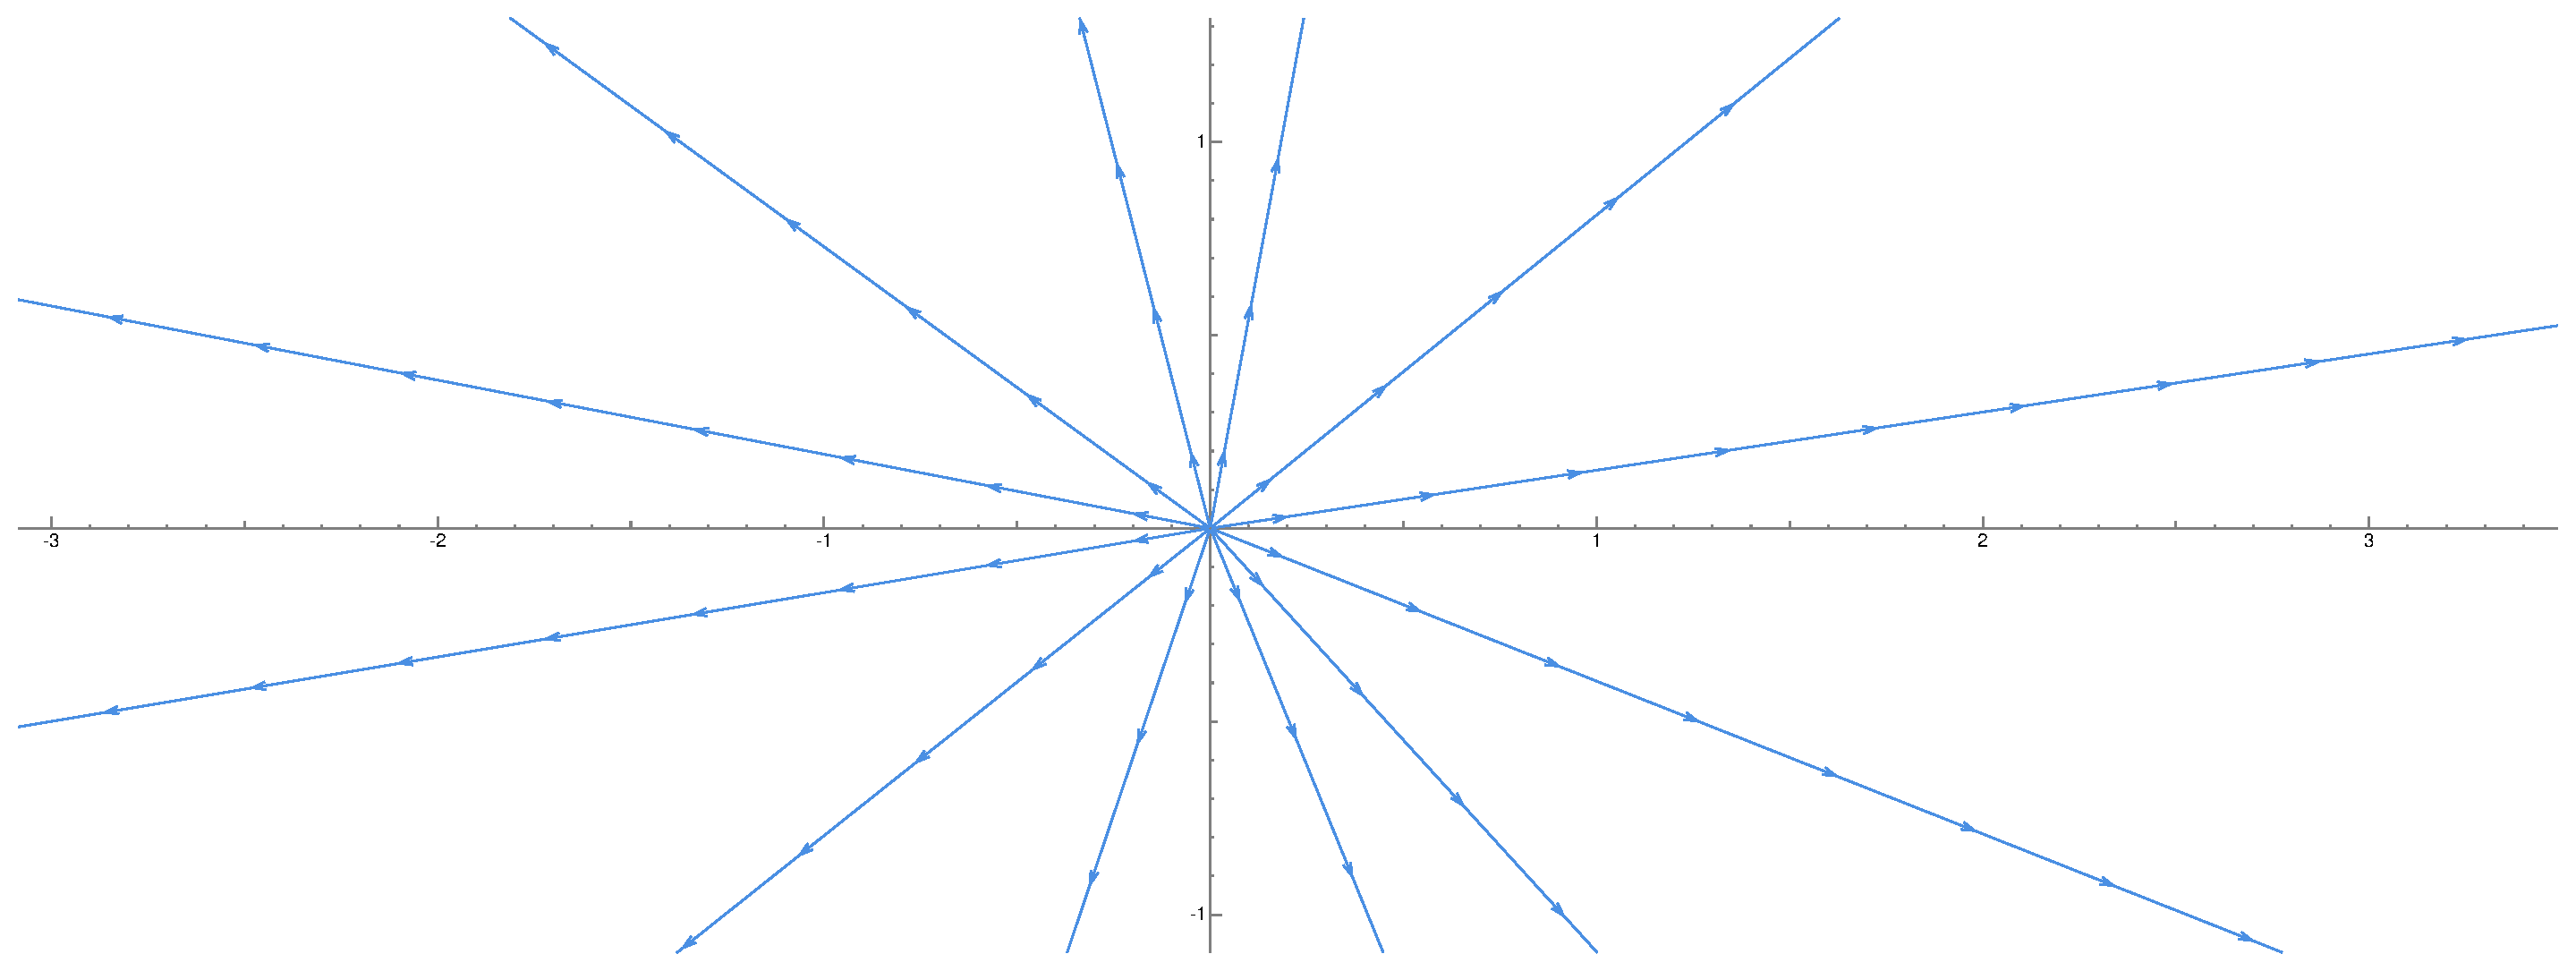
\includegraphics[width=11cm]{Immagini/stella_instabile.pdf}
    \caption{Stella instabile}
\end{figure}


\begin{figure}[!htb]
    \centering
    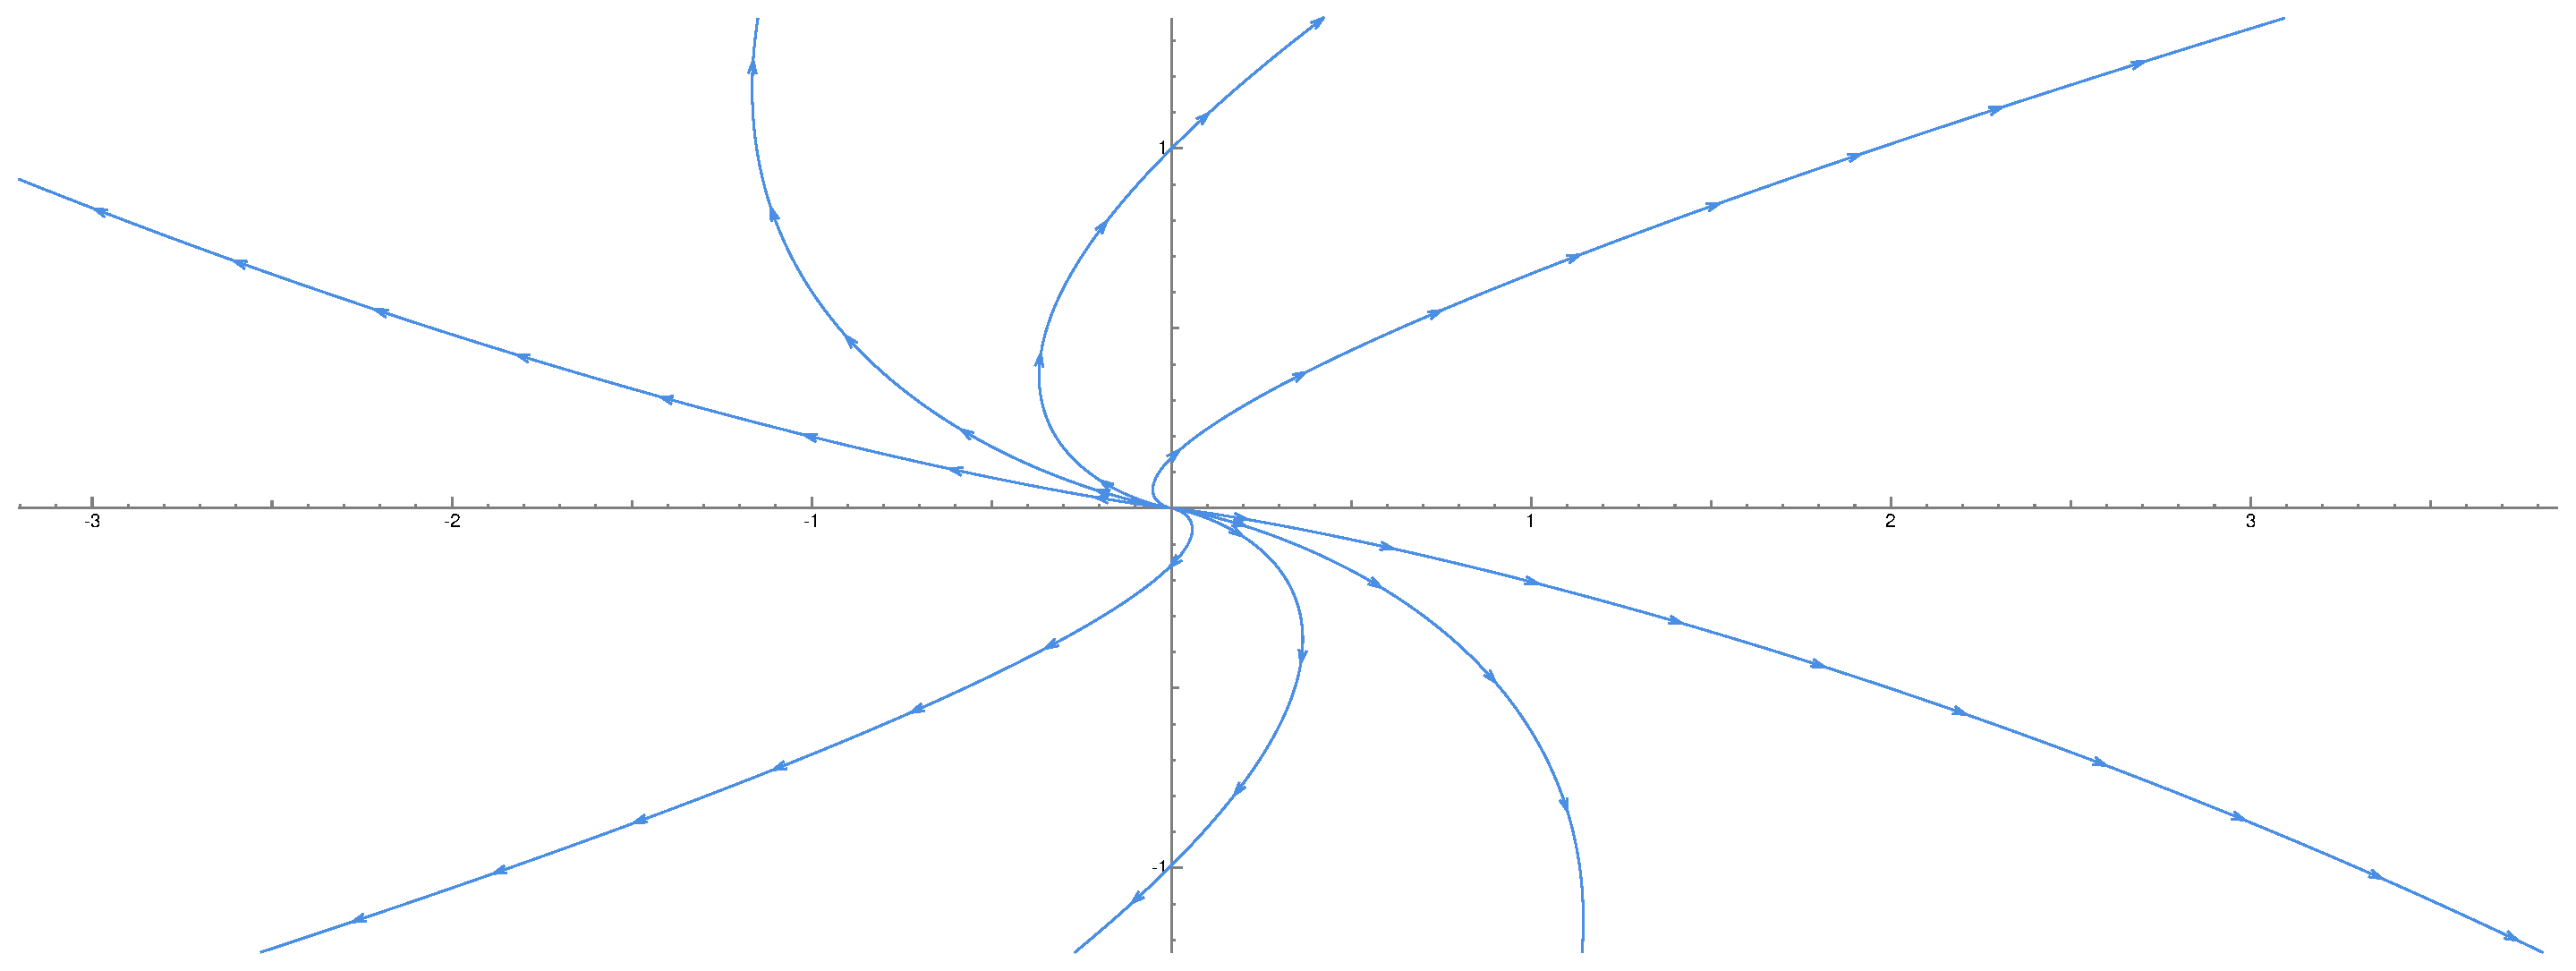
\includegraphics[width=11cm]{Immagini/nodo_improprio_instabile.pdf}
    \caption{Nodo improprio instabile}
\end{figure}


\begin{figure}[!htb]
    \centering
    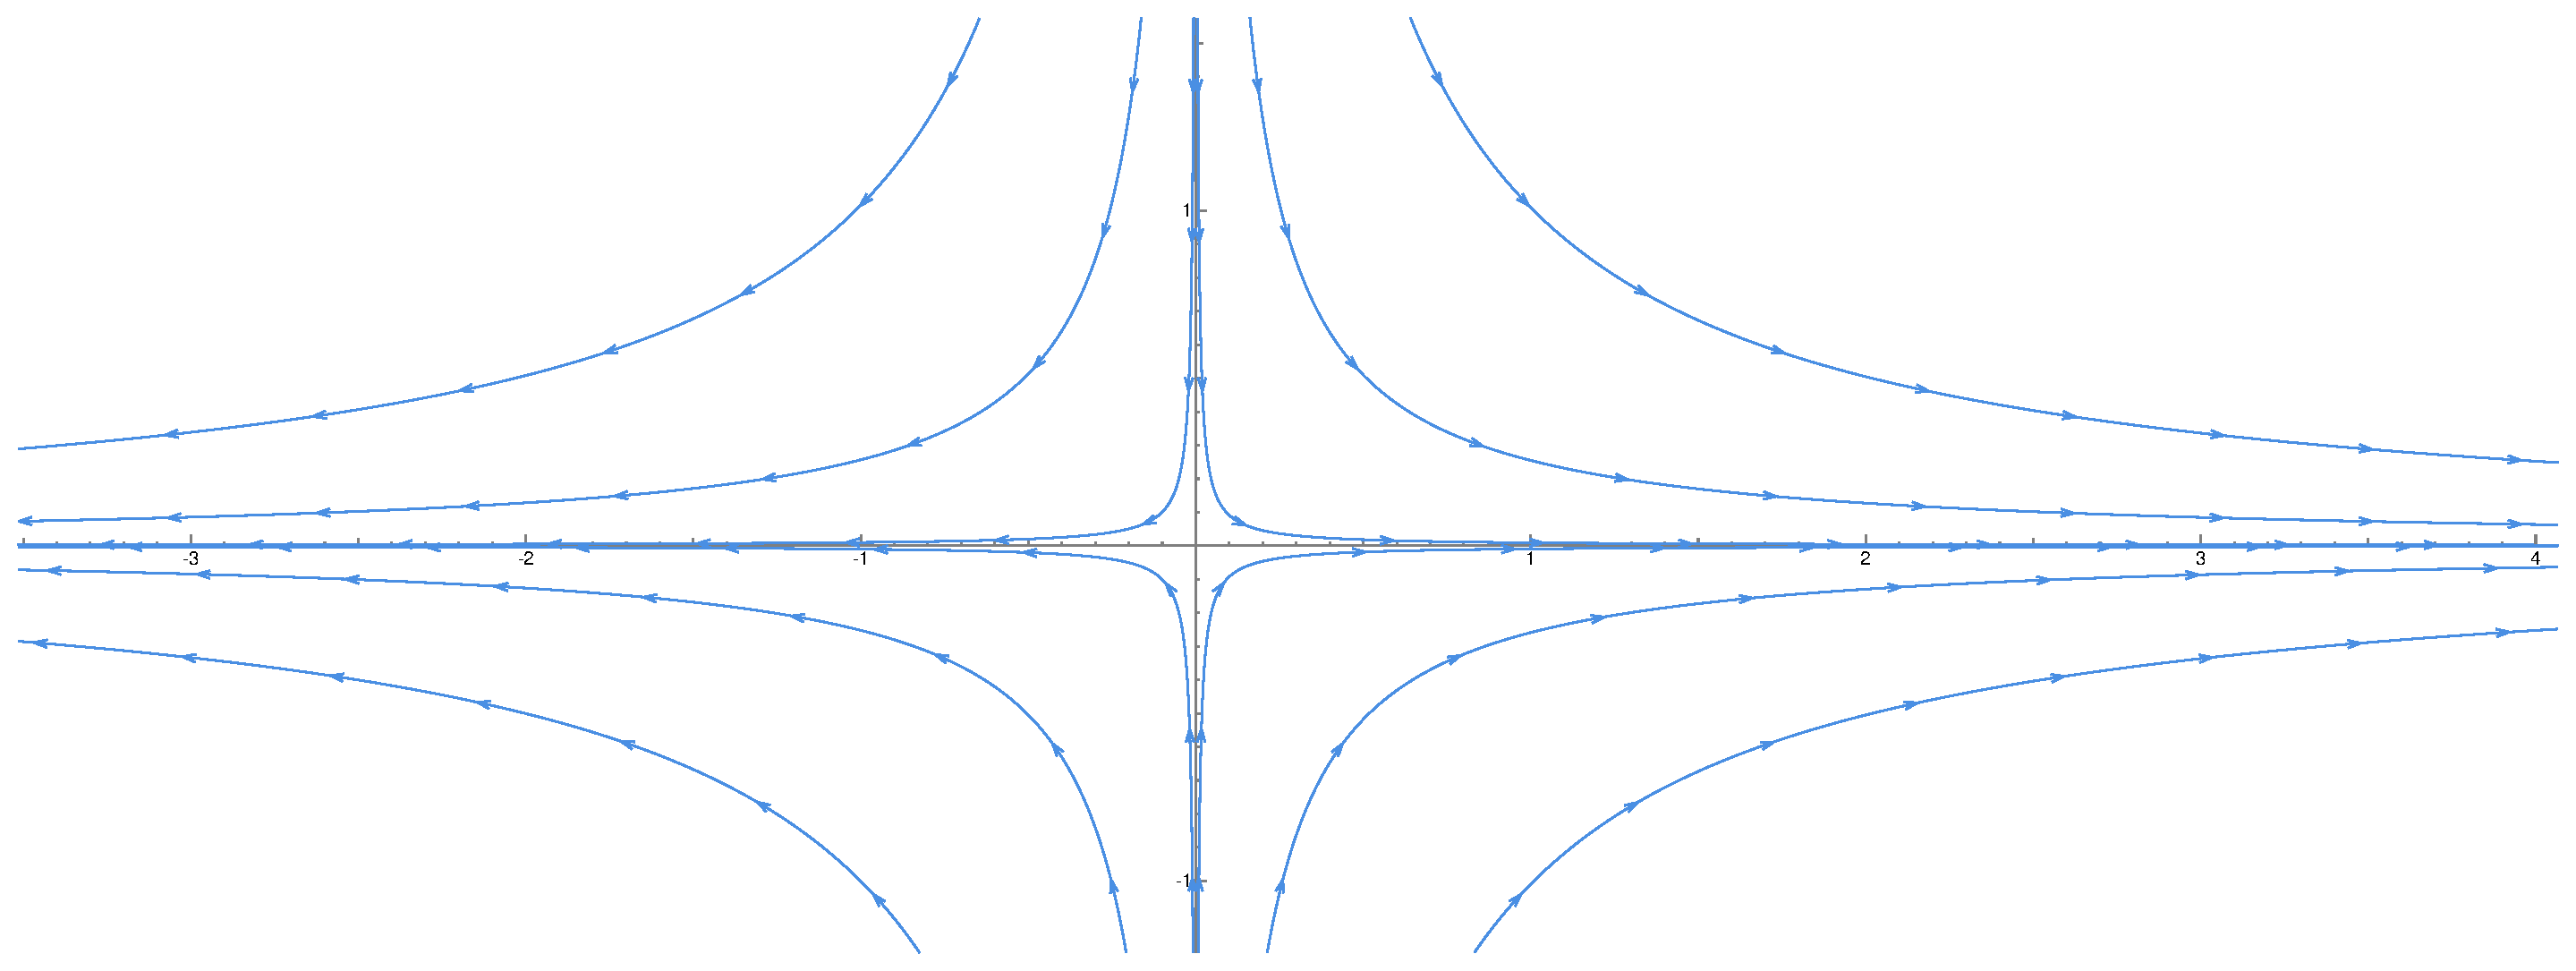
\includegraphics[width=11cm]{Immagini/sella.pdf}
    \caption{Sella}
\end{figure}


\begin{figure}[!htb]
    \centering
    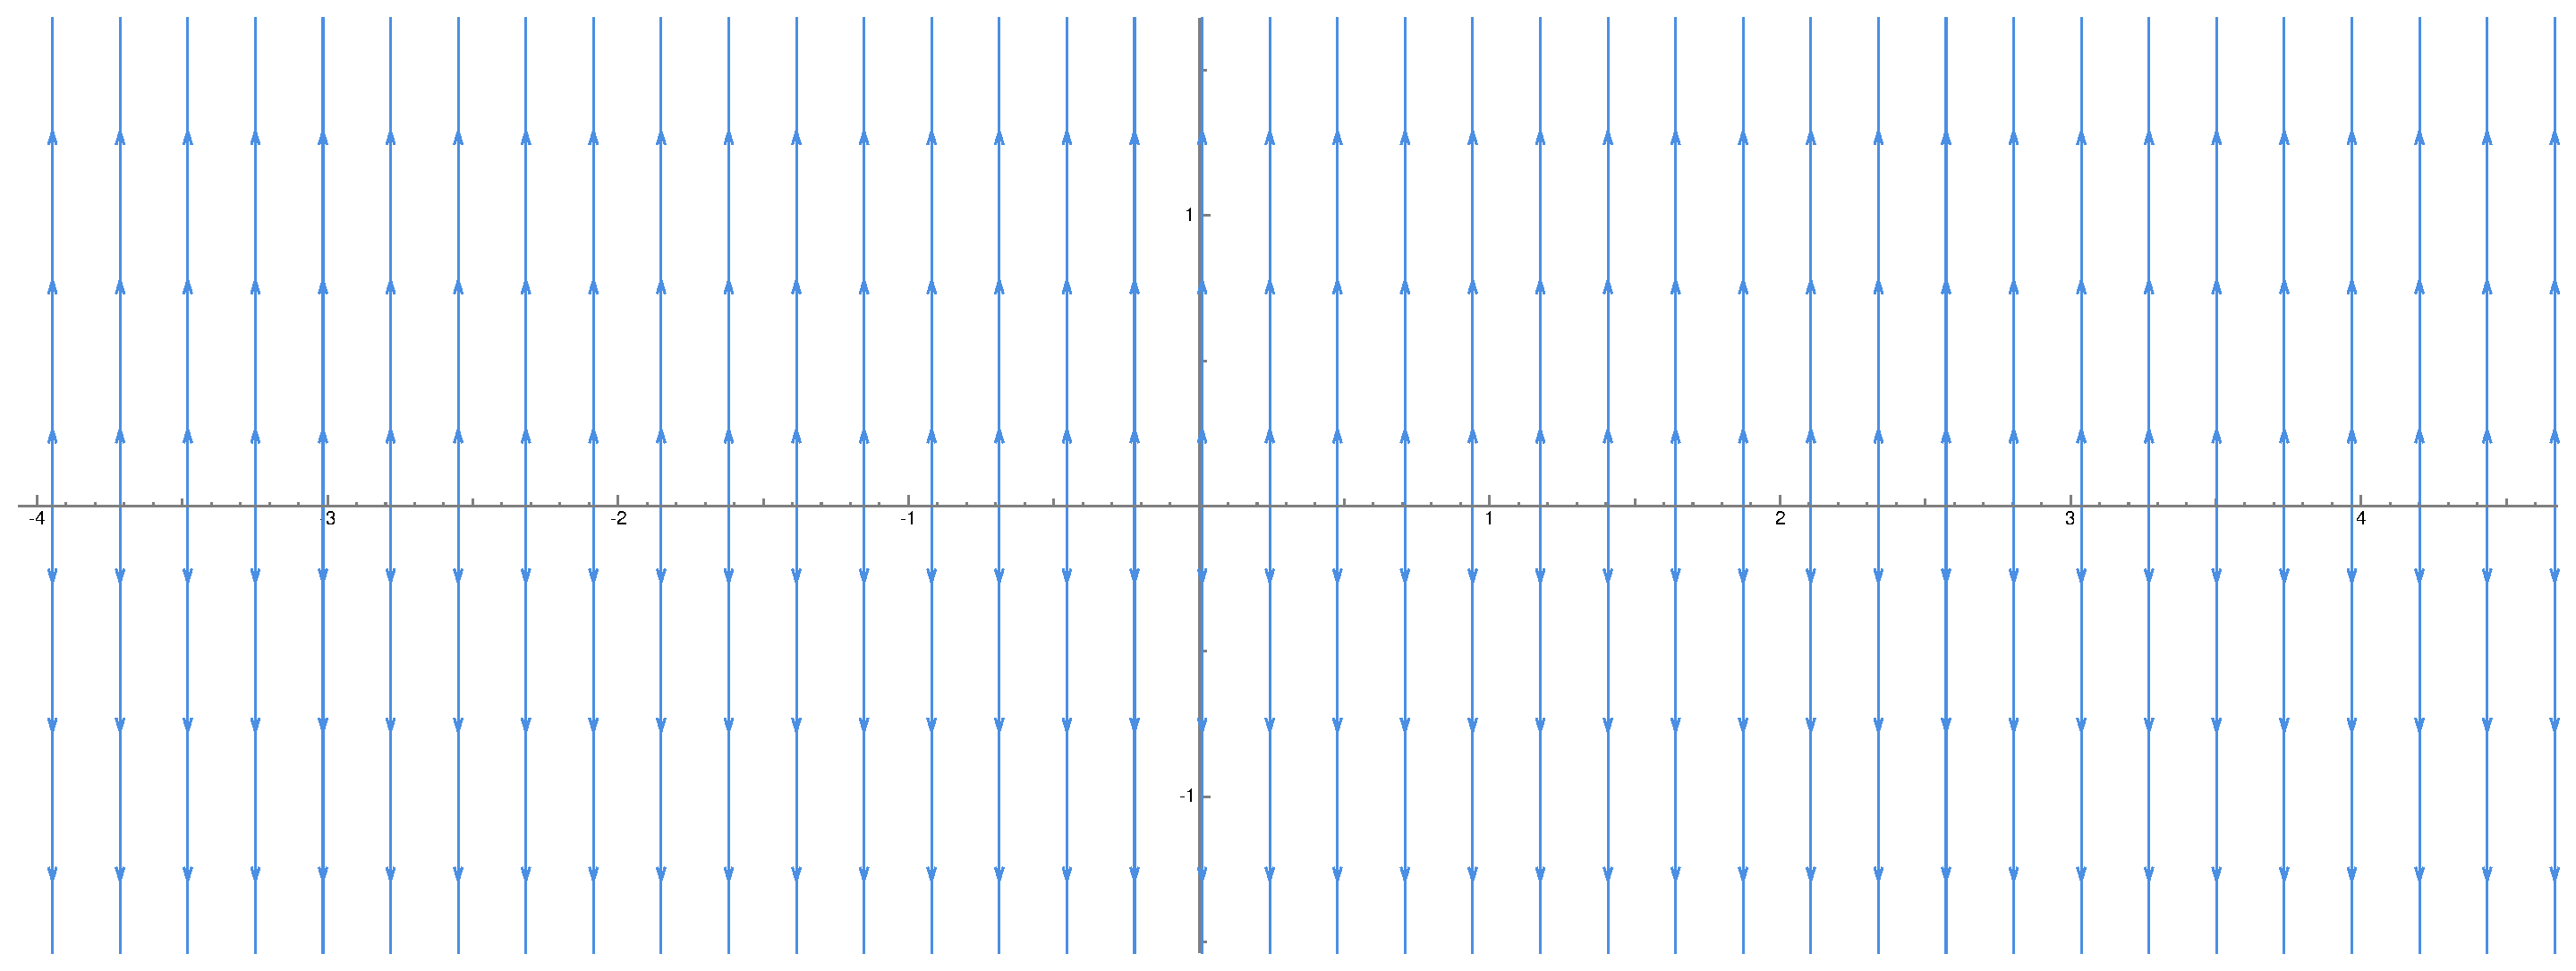
\includegraphics[width=11cm]{Immagini/rette_diagonale.pdf}
    \caption{Rette per matrice diagonalizzabile}
\end{figure}


\begin{figure}[!htb]
    \centering
    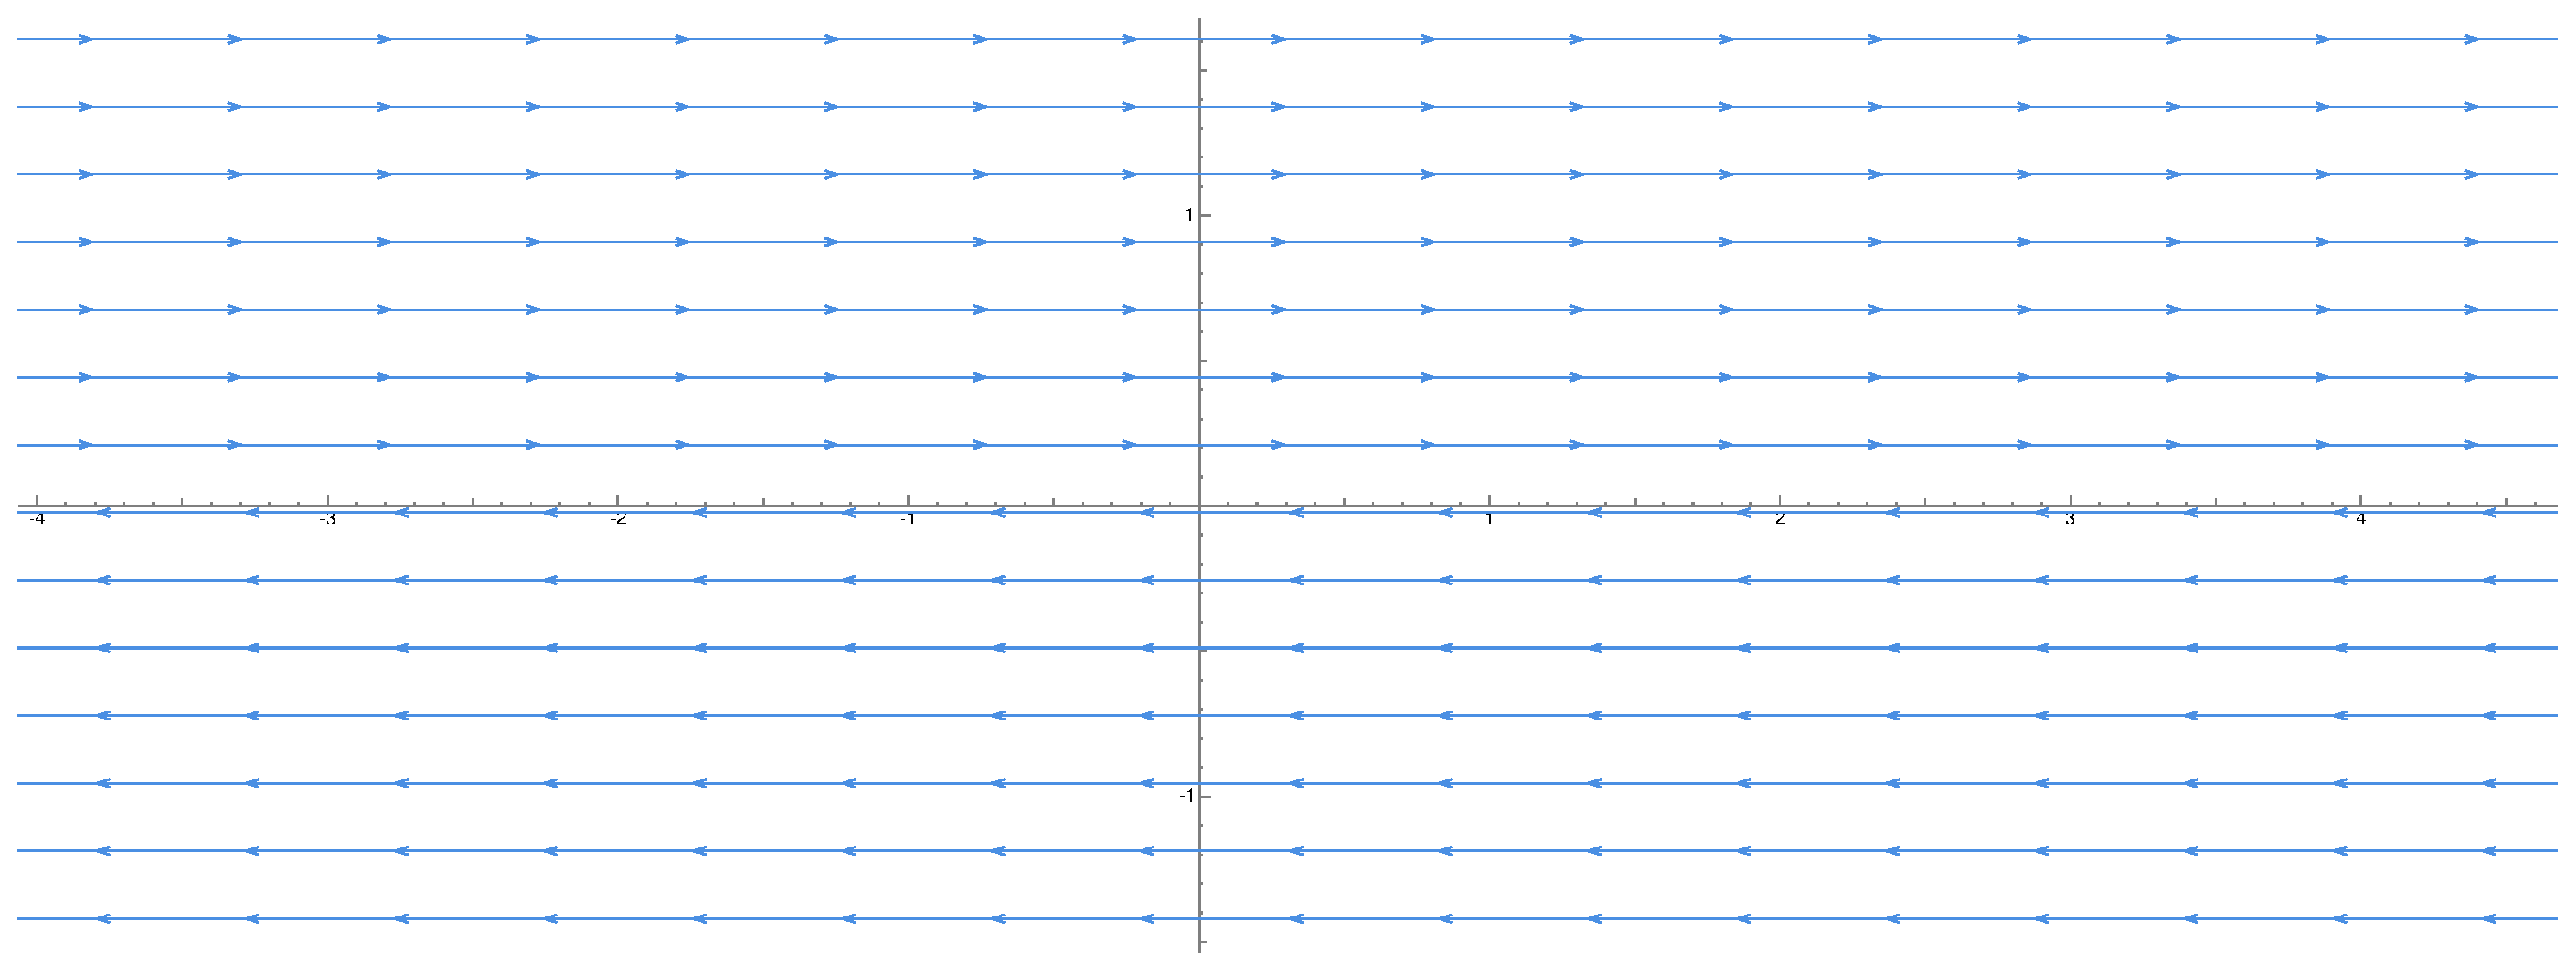
\includegraphics[width=11cm]{Immagini/rette_jordan.pdf}
    \caption{Rette per blocco di Jordan nilpotente}
\end{figure}




